The anomalous Hall effect refers to the appearance of a large spontaneous Hall current in ferromagnet in response to an electric field alone \cite{vanderbilt2018berry}, and it was first discovered by Hall in 1881 \cite{hall1881}. Despite its century long history and importance, the microscopic characterization of the anomalous Hall effect has been a controversial subject. In the past three main mechanisms have been identified:
\begin{itemize}
    \item Berry curvature induced Hall effect \cite{karplus1954hall}
    \item Skew scattering \cite{smith1958resonant}
    \item Side-jump scattering \cite{berger1970side}
\end{itemize}

The Berry curvature induced Hall effect can be regarded as an \textit{intrinsic contribution} to the conductivity, the other two are regarded as \textit{extrinsic contributions}, this is because they are related to some kind of asymmetry to the scattering with impurities. More precisely the skew scattering deals with the asymmetry that arises with spin-orbit coupling between the electrons and the impurity, while the side jump is a sudden shift in of the electron coordinates during scattering \cite{berger1970side}. The effects are illustrated in figure \ref{fig:anomalous-contributions}.
\begin{figure}
    \centering
    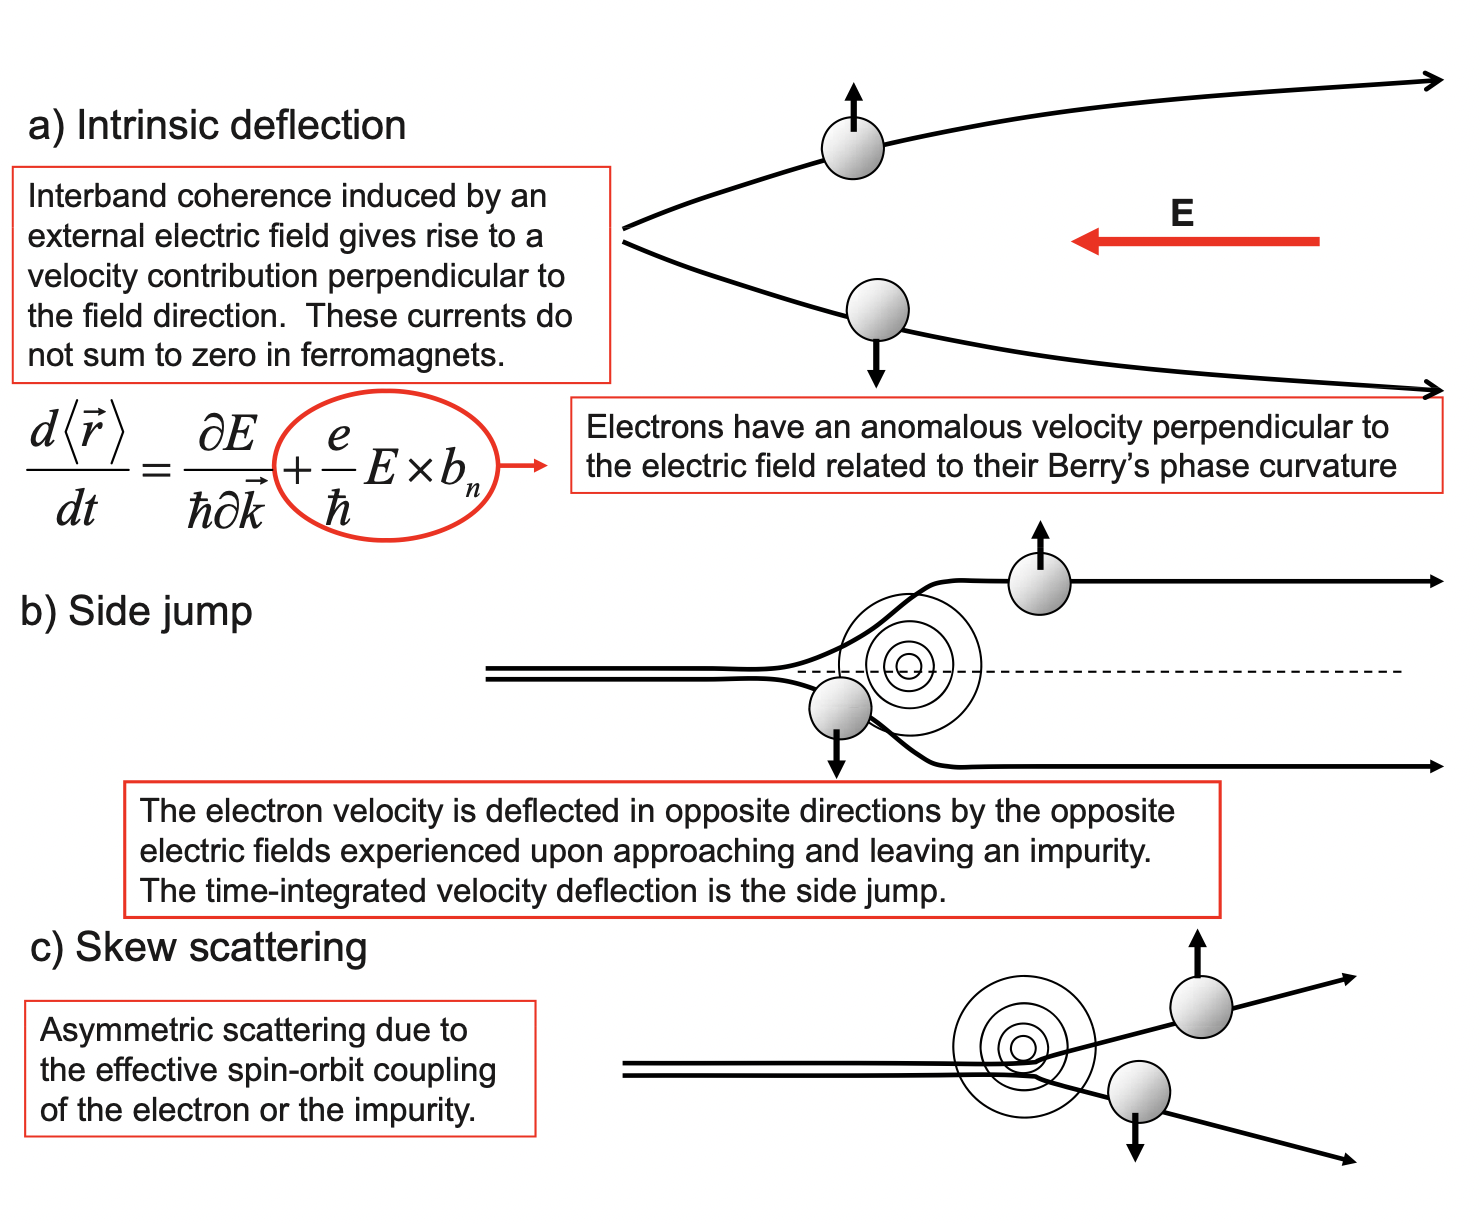
\includegraphics[width=.7\linewidth]{Immagini/ValleyHall/anomalous.png}
    \caption{All three contributions to the anomalous Hell effect, as you can see the intrinsic contribution does not need an impurity to scatter from. Image taken from \cite{nagaosa2010anomalous}}
    \label{fig:anomalous-contributions}
\end{figure}
The total Hall conductivity is the sum of all three contributions
\begin{equation}
    \sigma_H=\sigma_H^\textrm{in}+\sigma_H^\textrm{sk}+\sigma_H^\textrm{sj}
\end{equation}
where $\sigma_H^\textrm{in}$ is the intrinsic contribution given from equation \ref{eq:fermi-cond}, $\sigma_H^\textrm{sk}$ is the skew scattering term, which is proportional to the relaxation time $\tau$, and $\sigma_H^\textrm{sj}$ is the side-jump term that is independent of $\tau$.

An important question is to identify the dominant contribution to the anomalous Hall effect (AHE). The way to compare theoretically the magnitude of the contribution rely mainly on semiclassical conduction theory \cite{dugaev2005anomalous}, and they express the dominance of the Berry induced Hall effect. In addition, a number of experimental results also gave favorable evidence for the dominance of the intrinsic contribution \cite{tian2009proper}. Because of this we are going to ignore $\sigma_H^\textrm{sk}$ and $\sigma_H^\textrm{sj}$.\\
To get used to the math used thought the whole thesis we'll calculate all the anomalous Hall effects exclusively in gapped graphene, however it can be done in several other materials with different hamiltonians.














